% Section propre à la version complète : comparaison entre plateformes
\section{Comparer les plateformes : ce que le corpus permet, et ce qu'il ne permet pas}
\label{sec:comparaison}

\subsection{Débit et puissance rapportés}

La figure~\ref{fig:fps-power} place toutes les lignes de \texttt{benchmarks.csv} qui ont à
la fois un \glslink{fps}{FPS} et une puissance : 82 sur 299, dont 53 sur FPGA. Elle se lit avec
prudence. Les tâches, les modèles et les résolutions diffèrent d'un point à l'autre. Les
points pleins ont une puissance mesurée (sur la puce ou la carte) ; les points creux, une
puissance estimée ou de portée inconnue.

\begin{figure}[!htbp]
\centering
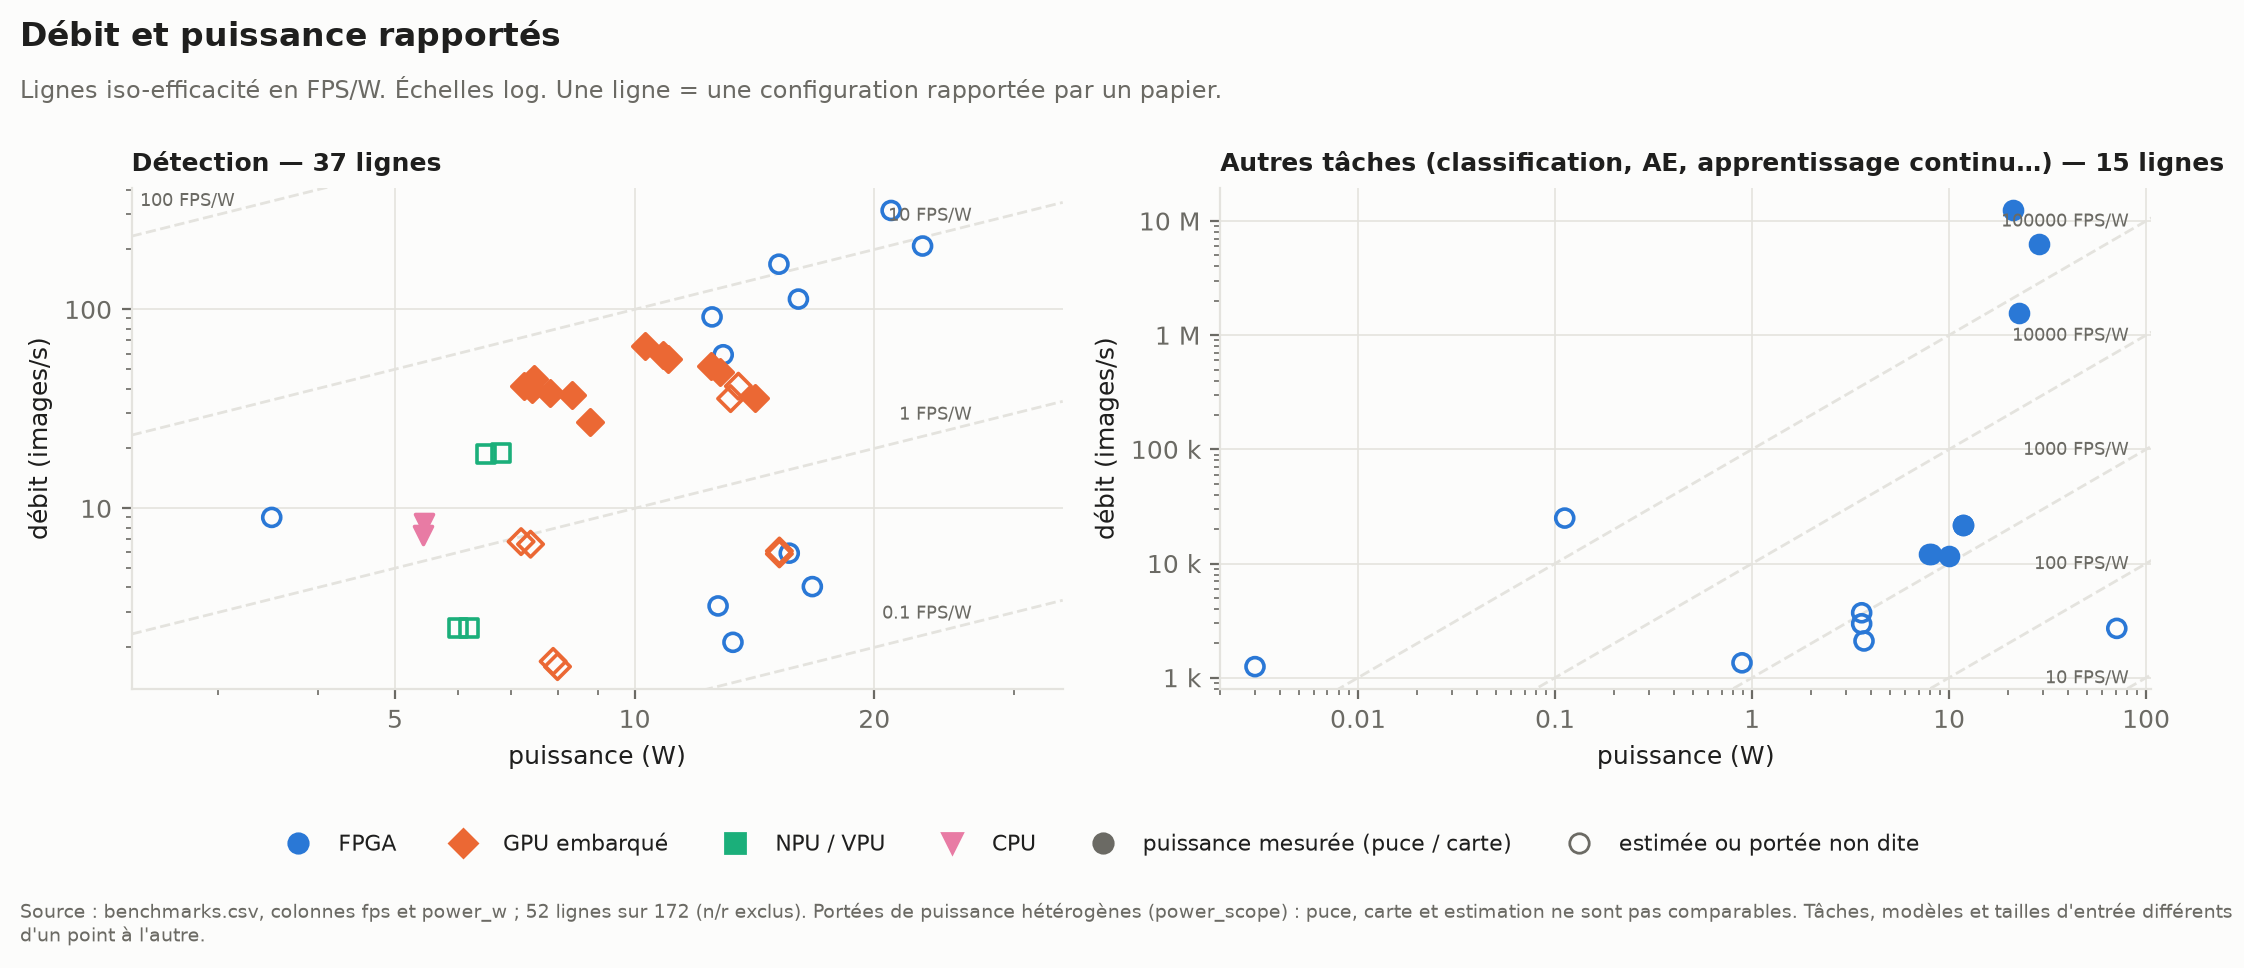
\includegraphics[width=\textwidth]{../../figures/bench_fps_power.png}
\caption{Débit et puissance rapportés, en échelles logarithmiques ; les droites
pointillées sont des lignes d'iso-efficacité en FPS/W. Figure générée par
\texttt{bin/pdb plot} à partir de \texttt{benchmarks.csv} (01/10/2026, 82 lignes sur 299).}
\label{fig:fps-power}
\end{figure}

Pour la détection (panneau de gauche, 50 lignes), ce que la figure montre :
\begin{itemize}
  \item les GPU \glslink{jetson}{Jetson} se regroupent entre 7 et 15\,\glslink{u-w}{W}, de 1,6 à 67\,images par seconde.
    Les points pleins sont les \glslink{orin-nano}{Orin Nano} et \glslink{orin-nx}{Orin NX} de Rey et al., mesurés par télémétrie
    embarquée \citep[Table~4]{arxiv-2502.15737-performance-analysis-you-only-look} ; les
    points creux, les \glslink{jetson-nano}{Jetson Nano} et \glslink{xavier-nx}{Xavier NX} de Feng et al., sans TensorRT et de portée
    non décrite \citep[Table~3]{2022-feng-benchmark-analysis-yolo-performance-edge} ;
  \item les FPGA s'étalent sur deux ordres de grandeur de débit (de 2,1 à 314\,\glslink{fps}{FPS}) et sur
    un ordre de grandeur de puissance (de 2 à 23\,\glslink{u-w}{W}) ;
  \item seules 7 des 23 lignes FPGA de détection ont une puissance mesurée, toutes au
    niveau de la carte : six \glslink{lp-yolo}{LP-YOLO} sur \glslink{pynq-z1}{PYNQ-Z1}, de 2,00 à 2,91\,\glslink{u-w}{W} pour 12 à 44\,\glslink{fps}{FPS}
    \citep[§V]{arxiv-2609.24757-npu-accelerator-quantized-real-time}\pp, et \glslink{codenet}{CoDeNet} sur
    \glslink{ultra96}{Ultra96}, 32,2\,\glslink{fps}{FPS} à 5,6\,\glslink{u-w}{W}
    \citep[Table~3]{arxiv-2006.08357-codenet-efficient-deployment-input-adaptive}$^{m}$.
    Les 16 autres sont estimées par Vivado ou de portée inconnue.
\end{itemize}
Ce que la figure ne permet pas : conclure qu'une famille est plus efficace qu'une autre.
Aucun couple de points ne partage à la fois le modèle, la résolution, la précision
numérique et la méthode de mesure \deduit. Les petites FPGA mesurées à 2--3\,\glslink{u-w}{W} portent des
\glslink{lp-yolo}{LP-YOLO} à 256 ou 320 pixels, filtrés sur les véhicules ; les \glslink{orin}{Orin} portent des \glslink{yolov8}{YOLOv8} à
640 pixels.

\subsection{Les comparaisons à tâche égale}

Six articles comparent une FPGA et un GPU embarqué sur le même réseau, mesurés par les
mêmes auteurs (table~\ref{tab:face-a-face}). Deux protocoles plus anciens s'y ajoutent :
fpgaConvNet face à un Tegra~X1 bridé à 76,8\,\glslink{u-mhz}{MHz} pour égaliser le budget de puissance
\citep[§3.1]{arxiv-1711.08740-fpgaconvnet-toolflow-mapping-diverse-convolutional}, et
\glslink{dac-sdc}{DAC-SDC}~2018, mesuré par les organisateurs \citep{2021-xu-dac-sdc-low-power-object}.

\begin{table}[!htbp]
\centering\footnotesize
\caption{Comparaisons FPGA contre GPU embarqué à réseau égal, dans un même article. Les
énergies marquées \deduit{} sont calculées ici (puissance divisée par le débit, ou
inverse du FPS/W publié).}
\label{tab:face-a-face}
\begin{tabularx}{\textwidth}{@{}P{2.3cm}P{2.4cm}LLP{3.2cm}@{}}
\toprule
Travail & Tâche, modèle & FPGA & GPU embarqué & Réserves \\
\midrule
\glslink{skynet}{SkyNet}\pp{} \src{Tables~5--7} & détection mono-objet, \glslink{dac-sdc}{DAC-SDC}'19 &
  \glslink{ultra96}{Ultra96}, FM9/W11 : \glslink{iou}{IoU} 0,716 ; 25,05\,\glslink{fps}{FPS} ; 7,26\,\glslink{u-w}{W} ; $\approx$\,0,29\,\glslink{u-j}{J}/image \deduit &
  \glslink{tx2}{TX2}, FP32 : \glslink{iou}{IoU} 0,731 ; 67,33\,\glslink{fps}{FPS} ; 13,50\,\glslink{u-w}{W} ; $\approx$\,0,20\,\glslink{u-j}{J}/image \deduit &
  portée \nr{} (organisateurs) ; batch~4 sur FPGA \\
Schlosser \src{Table~1} & \glslink{yolov4}{YOLOv4} 512, COCO &
  \glslink{zcu104}{ZCU104}, \glslink{dpu}{DPU} INT8 : \glslink{map}{mAP} 37,5 ; 54,42\,\glslink{u-ms}{ms} ; 23\,\glslink{u-w}{W} ; 1,31\,\glslink{fpsw}{FPS/W} &
  \glslink{agx-xavier}{AGX Xavier}, TensorRT INT8 : \glslink{map}{mAP} 38,6 ; 22,0\,\glslink{u-ms}{ms} ; 16,5\,\glslink{u-w}{W} ; 2,05\,\glslink{fpsw}{FPS/W} &
  carte au multimètre des deux côtés ; post-traitement optimisé sur \glslink{dpu}{DPU}, en Python sur
  \glslink{jetson}{Jetson} \\
SATAY \src{Table~IV}$^{m}$ & \glslink{yolov5n}{YOLOv5n} 640 & \glslink{zcu104}{ZCU104} : 317\,\glslink{u-mj}{mJ} & \glslink{tx2}{TX2} : 277\,\glslink{u-mj}{mJ} &
  méthode \nr ; en 320, \glslink{tx2}{TX2} 70,7\,\glslink{u-mj}{mJ} contre 117,5 à 431\,\glslink{u-mj}{mJ} \\
Castelino \src{Table~VI, §IV-B}$^{m}$ & \glslink{cae}{CAE} d'anomalies, images hyperspectrales &
  \glslink{zcu104}{ZCU104}, \glslink{dpu}{DPU} INT8 : \glslink{f1}{F1} 92,77 ; 4,0\,\glslink{u-ms}{ms} ; 5,38\,\glslink{u-w}{W} ; 21,52\,\glslink{u-mj}{mJ} &
  \glslink{xavier-nx}{Xavier NX} 10\,\glslink{u-w}{W}, TensorRT INT8 : \glslink{f1}{F1} 95,29 ; 10,36\,\glslink{u-ms}{ms} ; 7,6\,\glslink{u-w}{W} ; $\approx$\,79\,\glslink{u-mj}{mJ}
  \deduit & puce (PMBus) contre jtop ; \glslink{jetson}{Jetson} bridée \\
\glslink{f-lic}{F-LIC} \src{Fig.~6}$^{m}$ & compression apprise, encodage 720p & \glslink{vcu118}{VCU118} : 1,41\,\glslink{u-j}{J} &
  \glslink{xavier-nx}{Xavier NX} : 1,43\,\glslink{u-j}{J} & méthode \nr ; grosse FPGA \\
\glslink{chameleon}{Chameleon} \src{Table~VI}$^{m}$ & apprentissage continu, \glslink{mobilenet}{MobileNetV1}, CORe50 &
  \glslink{zcu102}{ZCU102}, FP16 : 413\,\glslink{u-ms}{ms} ; 1,22\,\glslink{u-j}{J} par image &
  \glslink{jetson-nano}{Jetson Nano} : 33\,\glslink{u-ms}{ms} ; 0,31\,\glslink{u-j}{J} par image & batch~1 contre 8 ; méthode \nr \\
\bottomrule
\end{tabularx}
\end{table}

Les sources : \citet{arxiv-1909.09709-skynet-hardware-efficient-method-object}\pp,
\citet{arxiv-2304.11580-framework-benchmarking-real-time-embedded},
\citet{2023-montgomerie-corcoran-satay-streaming-architecture-toolflow-accelerating},
\citet{arxiv-2407.17647-energy-efficient-artefact-detection-accelerator},
\citet{2022-sun-f-lic-fpga-learned-image} et
\citet{2024-aggarwal-chameleon-dual-memory-replay-online}. Ce que la table montre :
\begin{itemize}
  \item sur les trois détecteurs, le GPU embarqué est au moins aussi sobre par image.
    Chez \glslink{skynet}{SkyNet}\pp{} et Schlosser et al., il est aussi plus rapide et plus précis, y
    compris en INT8 des deux côtés : le \glslink{yolov4}{YOLOv4} de Schlosser et al. tient 2,05\,\glslink{fpsw}{FPS/W} sur
    \glslink{agx-xavier}{AGX Xavier} contre 1,31 sur \glslink{zcu104}{ZCU104}. SATAY est en moyenne 3,6 fois plus rapide que la
    \glslink{tx2}{TX2} \src{§VI-B}, mais pas plus sobre ;
  \item la seule comparaison favorable au FPGA est celle de Castelino et al. : 2,6 fois
    moins de latence et 3,6 fois moins d'énergie que la \glslink{xavier-nx}{Xavier NX} \src{§IV-B}. Mais les
    portées diffèrent (rails de la puce contre jtop), la \glslink{jetson}{Jetson} est bridée à 10\,\glslink{u-w}{W}, et le
    FPGA perd 2,5 points de \glslink{f1}{F1}. Il s'agit d'un \glslink{ae}{autoencodeur}, pas d'un détecteur ;
  \item \glslink{f-lic}{F-LIC} est à parité d'énergie avec la \glslink{xavier-nx}{Xavier NX}, sur une FPGA de centre de calcul ;
    \glslink{chameleon}{Chameleon} est quatre fois moins sobre que la \glslink{jetson-nano}{Jetson Nano} \deduit.
\end{itemize}
Aucune de ces comparaisons n'oppose une FPGA embarquée à une \glslink{orin}{Jetson Orin} \deduit.

\subsection{Énergie par inférence : des ordres de grandeur}

\begin{table}[!htbp]
\centering\footnotesize
\caption{Énergie par inférence (ou par événement d'apprentissage) rapportée dans le corpus.
Tâches, modèles et portées diffèrent : ces valeurs donnent des ordres de grandeur, pas un
classement. Les valeurs marquées \deduit{} sont calculées ici à partir de la puissance et
du débit publiés.}
\label{tab:energie}
\begin{tabularx}{\textwidth}{@{}P{2.6cm}LP{2.4cm}rP{2.8cm}@{}}
\toprule
Travail & Tâche, modèle & Plateforme & Énergie & Portée, source \\
\midrule
\glslink{tinyissimoyolo}{TinyissimoYOLO} & détection 88$\times$88, 3 classes & MAX78000 & 196\,\glslink{u-uj}{µJ} & MCU seul, §III \\
\glslink{tinyissimoyolo}{TinyissimoYOLO} & idem & Apollo4b & 6,1\,\glslink{u-mj}{mJ} & MCU seul, §III \\
Manjunath & encodeur \glslink{ae}{AE} 120$\times$120 & \glslink{artix7}{Artix-7} & 0,25\,\glslink{u-mj}{mJ} & estimée (Vivado), Table~5 \\
\glslink{imagehd}{ImageHD} & clustering continu, CIFAR-10 & \glslink{zcu104}{ZCU104} & 0,97\,\glslink{u-mj}{mJ} & estimée (Vitis), Table~VII \\
MLPerf Tiny\pp & classification CIFAR-10, FINN W1A1 & \glslink{pynq-z2}{Pynq-Z2} & 2,5\,\glslink{u-mj}{mJ} & appareil sous
  test (Joulescope), Table~5 \\
Castelino & \glslink{cae}{CAE} d'anomalies, hyperspectral & \glslink{zcu104}{ZCU104} & 21,5\,\glslink{u-mj}{mJ} & puce (PMBus), §IV-B \\
Castelino (baseline) & idem & \glslink{xavier-nx}{Xavier NX} (10\,\glslink{u-w}{W}) & $\approx$\,79\,\glslink{u-mj}{mJ} & jtop, Table~VI
  \deduit \\
\glslink{lp-yolo}{LP-YOLO Slim}\pp & détection de véhicules, 256 & \glslink{pynq-z1}{PYNQ-Z1} & $\approx$\,82\,\glslink{u-mj}{mJ} & carte
  (rail 12\,V), §V-D \deduit \\
Rey & \glslink{yolov8n}{YOLOv8n} 640 INT8 & \glslink{orin-nx}{Orin NX} & 179\,\glslink{u-mj}{mJ} & télémétrie, Table~4 \\
Rey & \glslink{yolov8n}{YOLOv8n} 640 INT8 & \glslink{orin-nano}{Orin Nano} & 185\,\glslink{u-mj}{mJ} & télémétrie, Table~4 \\
\glslink{skynet}{SkyNet}\pp & détection mono-objet & \glslink{tx2}{TX2} / \glslink{ultra96}{Ultra96} & $\approx$\,200 / 290\,\glslink{u-mj}{mJ} &
  \nr, Tables~5--6 \deduit \\
Karki\pp & \glslink{yolov26n}{YOLOv26n} 416 INT8 & \glslink{zcu104}{ZCU104} & $\approx$\,257\,\glslink{u-mj}{mJ} & estimée (Vivado),
  §IV-C, Table~III \deduit$^{m}$ \\
SATAY & \glslink{yolov5n}{YOLOv5n} 640 & \glslink{zcu104}{ZCU104} & 317\,\glslink{u-mj}{mJ} & non décrite, Table~IV$^{m}$ \\
SATAY (baseline) & \glslink{yolov5n}{YOLOv5n} 640 & \glslink{tx2}{Jetson TX2} & 277\,\glslink{u-mj}{mJ} & non décrite, Table~IV$^{m}$ \\
Schlosser & \glslink{yolov4}{YOLOv4} 512 INT8 & \glslink{agx-xavier}{AGX Xavier} / \glslink{zcu104}{ZCU104} & $\approx$\,0,49 / 0,76\,\glslink{u-j}{J} & carte,
  Table~1 \deduit \\
Alqahtani\pp & \glslink{yolov8}{YOLOv8} n à m, service web & \glslink{orin-nano}{Orin Nano} & 0,47 à 0,79\,\glslink{u-j}{J} & carte, repos
  soustrait, §IV \deduit$^{m}$ \\
\glslink{f-lic}{F-LIC} & encodage 720p (compression apprise) & \glslink{vcu118}{VCU118} & 1,41\,\glslink{u-j}{J} & non décrite, Fig.~6$^{m}$ \\
\glslink{f-lic}{F-LIC} (baseline) & idem & \glslink{xavier-nx}{Xavier NX} & 1,43\,\glslink{u-j}{J} & non décrite, Fig.~6$^{m}$ \\
\glslink{chameleon}{Chameleon} & image d'apprentissage continu & \glslink{zcu102}{ZCU102} / \glslink{jetson-nano}{Jetson Nano} & 1,22 / 0,31\,\glslink{u-j}{J} & non
  décrite, Table~VI$^{m}$ \\
O-FSCIL & ajout d'une classe (5 exemples) & \glslink{gap9}{GAP9} & 11,35\,\glslink{u-mj}{mJ} & non décrite, Table~IV \\
\glslink{qlr-cl}{QLR-CL} & événement d'apprentissage ($l = 27$) & \glslink{vega}{VEGA} & 0,13\,\glslink{u-j}{J} & puce, Table~IV \\
\glslink{qlr-cl}{QLR-CL} & idem & \glslink{stm32l4}{STM32L4} & 4,80\,\glslink{u-j}{J} & Table~IV \\
\bottomrule
\end{tabularx}
\end{table}

Sources des lignes nouvelles : MLPerf Tiny
\citep[Table~5]{arxiv-2206.11791-open-source-fpga-ml-codesign}\pp ; \glslink{lp-yolo}{LP-YOLO Slim}, 35,66\,\glslink{fps}{FPS}
à 2,91\,\glslink{u-w}{W}, soit 12,25\,\glslink{fpsw}{FPS/W}
\citep[§V-D]{arxiv-2609.24757-npu-accelerator-quantized-real-time}\pp ; Karki et al.,
34,05\,\glslink{fps}{FPS} de bout en bout et 8,760\,\glslink{u-w}{W} estimés par Vivado
\citep[§IV-C, Table~III]{arxiv-2607.13106-no-attention-no-problem-dpu}\pp ; Alqahtani et
al., 0,13 à 0,22\,mWh par requête, latence de service web comprise
\citep[§IV]{arxiv-2409.16808-comprehensive-evaluation-deep-learning-object}\pp. Pour
mémoire, le \glslink{yolov3-tiny}{YOLOv3-tiny} de Zhai et al. donnerait environ 136\,\glslink{u-mj}{mJ} par image (12,51\,\glslink{u-w}{W}
divisés par 91,65\,\glslink{fps}{FPS}, \citealp[Table~8]{2023-zhai-fpga-vehicle-detection-tracking-accelerator}),
de portée non décrite. Ces calculs sont les nôtres \deduit.

La table ne classe pas les plateformes. Trois écarts la dominent : la taille du réseau
(de 88$\times$88 pixels sur MCU à 640 sur \glslink{jetson}{Jetson}), la portée de la mesure (outil, puce,
carte, carte moins le repos), et le périmètre de l'inférence (noyau seul, bout en bout,
service web). Le seul détecteur sur petite FPGA mesuré à la carte (\glslink{lp-yolo}{LP-YOLO}, 82\,\glslink{u-mj}{mJ}) et
les \glslink{orin}{Orin} mesurés par télémétrie (179 à 185\,\glslink{u-mj}{mJ}) diffèrent sur ces trois points à la fois.

\subsection{Pourquoi la comparaison reste ouverte}

Pour comparer honnêtement un FPGA embarqué, une \glslink{jetson}{Jetson} et un MCU, il faudrait, sur un même
réseau :
\begin{itemize}
  \item la même précision numérique et le même batch ;
  \item une précision mesurée sur chaque cible ;
  \item une latence de bout en bout, post-traitement compris ;
  \item une puissance de puce et de carte, avec le repos mesuré.
\end{itemize}
Le protocole de \citet{arxiv-2304.11580-framework-benchmarking-real-time-embedded} est le
plus proche de cette grille dans le corpus : même \glslink{yolov4}{YOLOv4}, \glslink{map}{mAP} mesurée sur la cible par un
hôte séparé, puissance de carte absolue et relative (repos soustrait), quatre modes de
puissance \glslink{jetson}{Jetson} \src{§3, §4.1, §4.4}. Il lui manque l'égalité du post-traitement et une cible
récente, et il ne porte que sur un modèle. MLPerf Tiny fixe aussi un protocole (latence à
batch~1, énergie au Joulescope), mais l'article ne compare aucune autre plateforme
\citep[§1, §4.4]{arxiv-2206.11791-open-source-fpga-ml-codesign}\pp. Les meilleures
baselines \glslink{jetson}{Jetson} récentes (Rey, Alqahtani\pp) n'ont pas de FPGA. Les travaux FPGA récents
se comparent à des \glslink{jetson}{Jetson} anciennes ou bridées (SATAY, \glslink{skynet}{SkyNet}\pp, Castelino), à un GPU de
bureau \citep[Table~10]{2026-fata-low-cost-fpga-enhanced-cnn}, ou à rien (Karki\pp, \glslink{lp-yolo}{LP-YOLO}\pp). Aucun article du corpus ne met une FPGA
embarquée et une \glslink{orin}{Jetson Orin}, ni une FPGA et un MCU, dans un même banc d'essai.
